\documentclass[../main.tex]{subfiles}

\pagestyle{main}
\renewcommand{\chaptermark}[1]{\markboth{\chaptername\ \thechapter:\ #1}{}}
\setcounter{chapter}{14}

\begin{document}




\chapter{Partial Differentiation}
\section{Functions of Two or More Variables}
\begin{itemize}
    \item \textbf{Function} (from $D$ to $E^1$): A mapping that assigns a unique number $w$ to each point $(x_1,\dots,x_n)\in D\subset E^n$.
    \begin{itemize}
        \item We write $w=f(x_1,\dots,x_n)$ and say that $w$ is the value of the function $f$ at $(x_1,\dots,x_n)$.
    \end{itemize}
    \item \textbf{Continuous} (function $f(x,y)$): A function $f(x,y)$ such that $w\to w_0=f(x_0,y_0)$ as $(x,y)\to(x_0,y_0)$.
\end{itemize}



\section{The Directional Derivative: Special Cases}
\begin{figure}[h!]
    \centering
    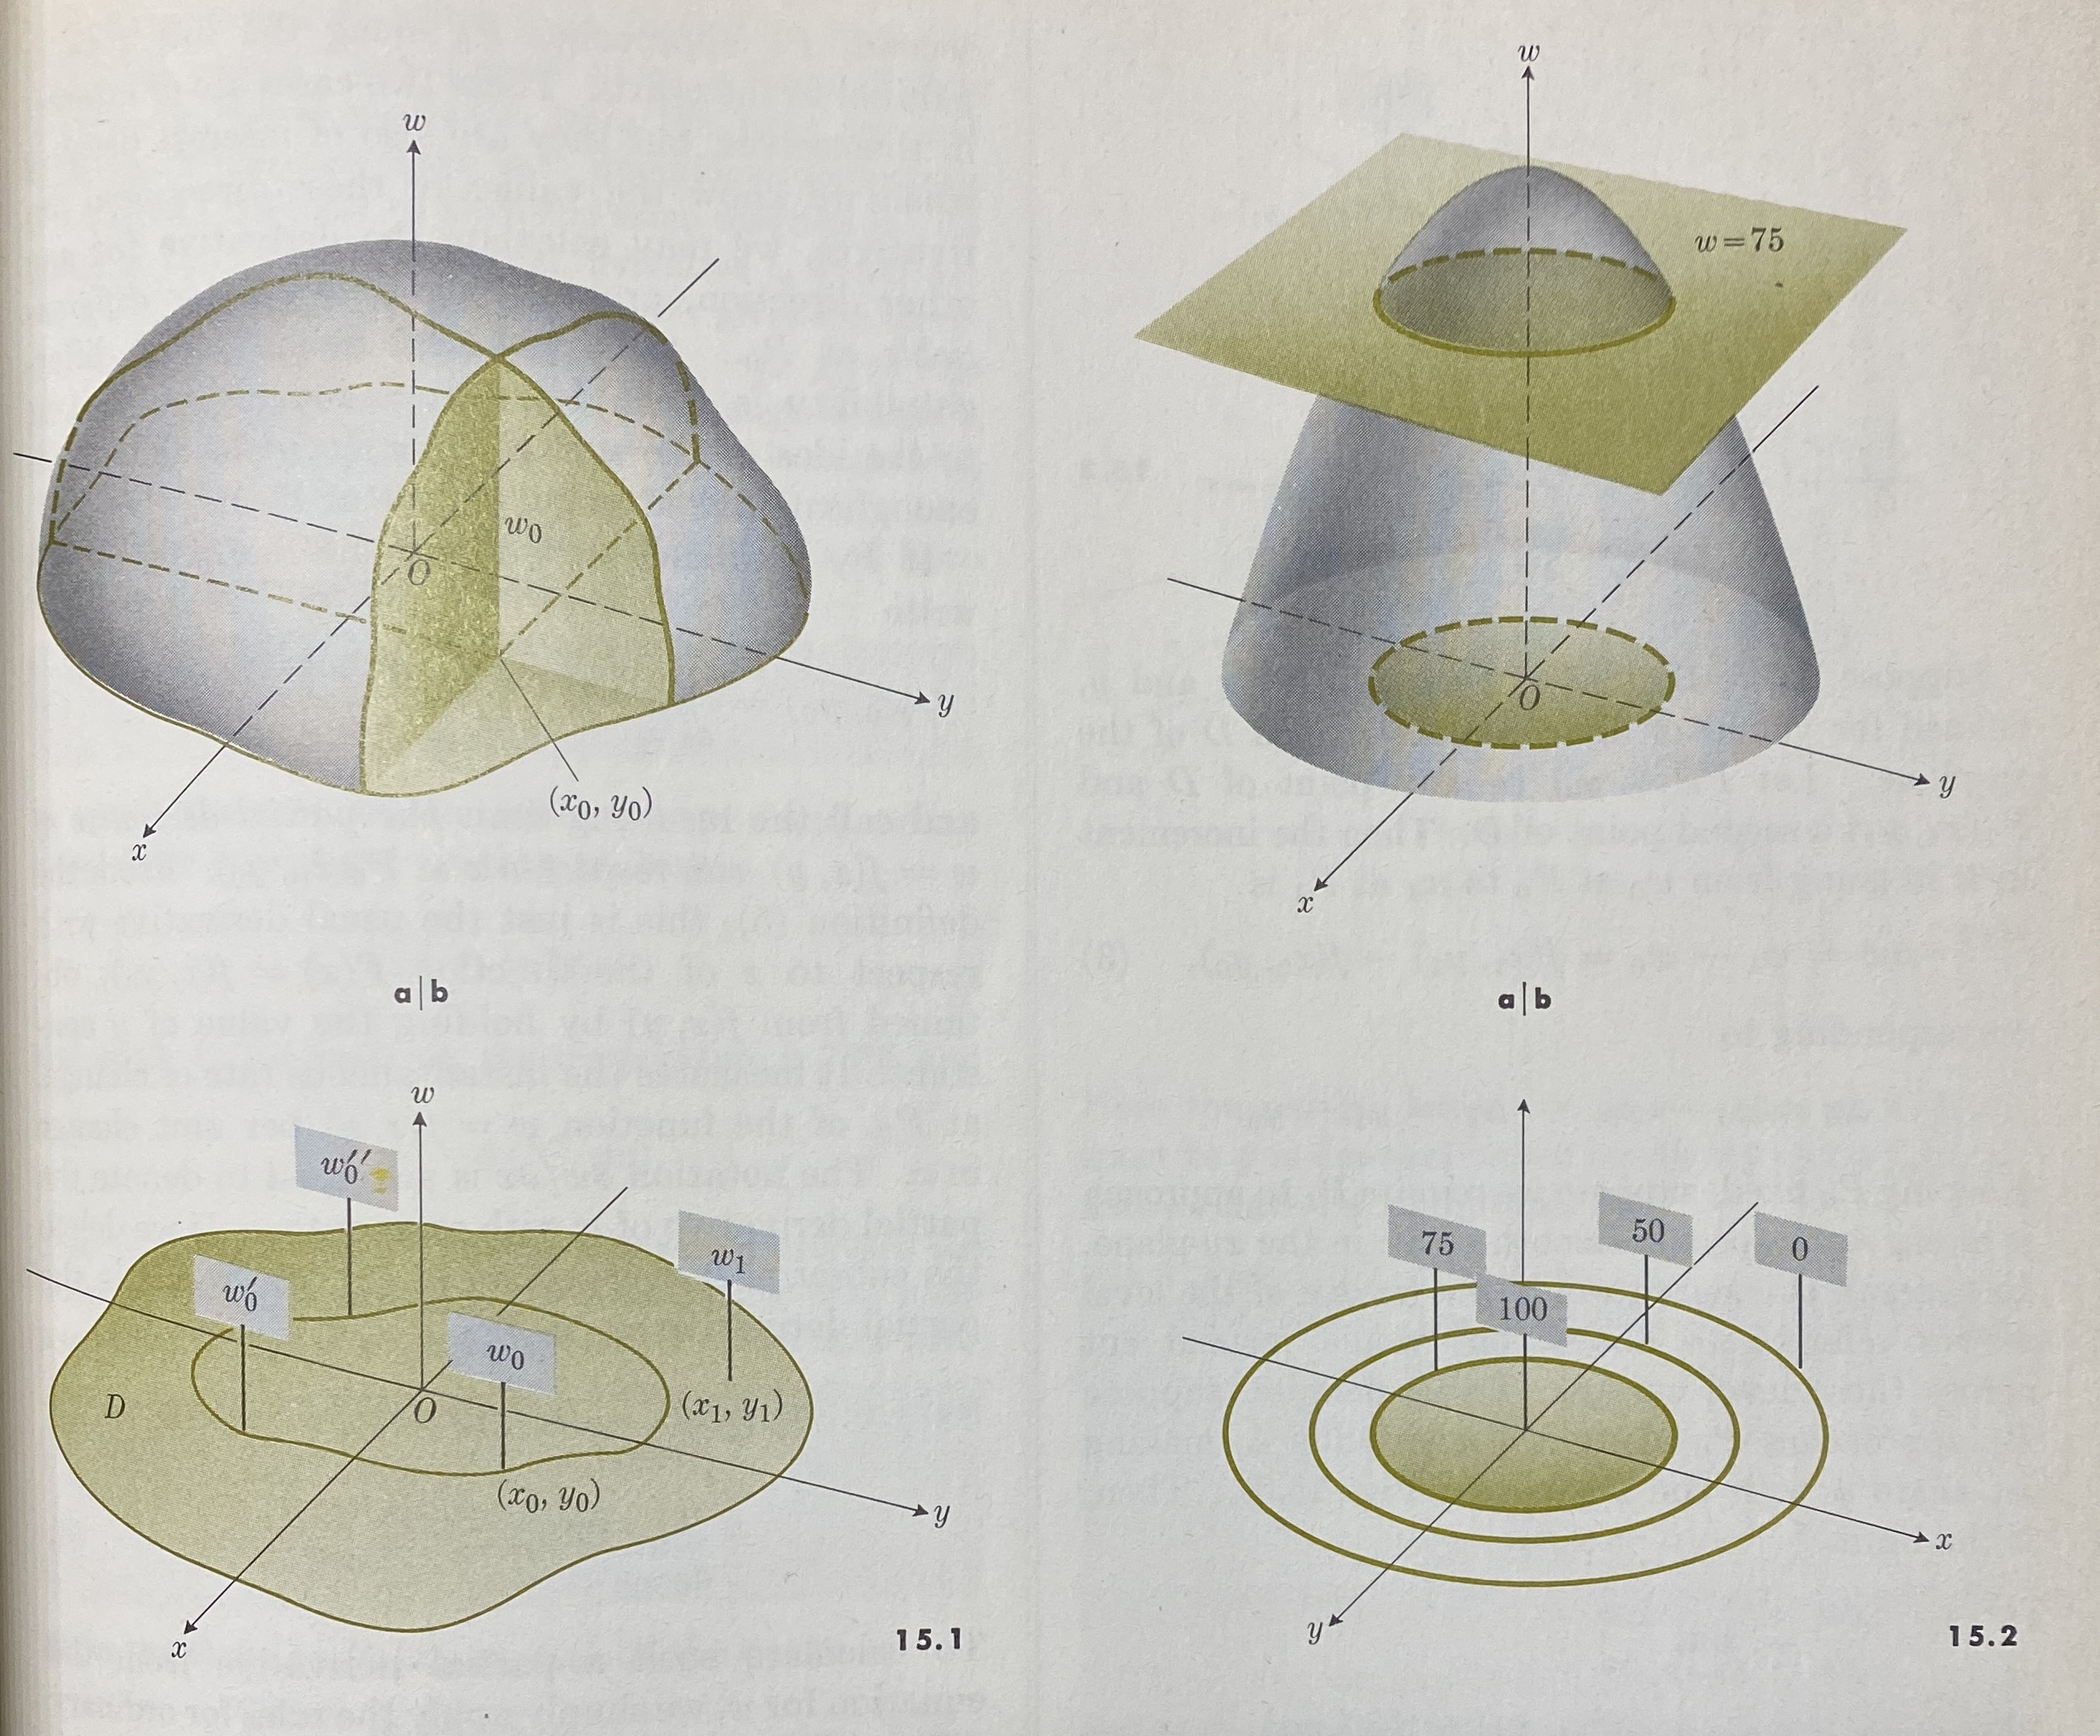
\includegraphics[width=0.7\linewidth]{ExtFiles/SurfacesAndContours.jpg}
    \caption{Surface plots and contour maps of 2D functions.}
    \label{fig:SurfacesAndContours}
\end{figure}
\begin{itemize}
    \item The equation $w=f(x,y)$ can be interpreted as representing a surface in $xyw$-space, or as a base region $D$ in the $xy$-plane with a marker bearing a corresponding $w$-value attached to each point.
    \begin{itemize}
        \item To introduce order into the second interpretation, we can construct a \textbf{contour map} with a number of \textbf{contour curves}.
    \end{itemize}
    \item \textbf{Contour curve}: A curve consisting of points $(x,y)\in D$ with equal $w$-values.
    \begin{itemize}
        \item The formula for such a curve can be derived by setting $w_0=f(x,y)$, where $w_0\in R_f$.
    \end{itemize}
    \item \textbf{Directional derivative} (of $f(x,y)$ at $(x_0,y_0)$ in the direction of $L$): The limit
    \begin{equation*}
        \dv{w}{s} = \lim_{\Delta s\to 0}\frac{\Delta w}{\Delta s} = \lim_{P_1\to P_0}\frac{f(x_1,y_1)-f(x_0,y_0)}{\sqrt{\Delta x^2+\Delta y^2}}
    \end{equation*}
    \begin{figure}[h!]
        \centering
        \begin{tikzpicture}[
            every node/.append style={black}
        ]
            \footnotesize
            \draw [->] (-0.5,0) -- (5,0) node[right]{$x$};
            \draw [->] (0,-0.6) -- (0,4) node[above]{$y$};
            \node [anchor=north east] {$O$};

            \draw [ylx,thick] (0.4,0.3) coordinate (A) -- node[above]{$L$} (4.5,3.5) coordinate (B);
            \fill ($(A)!0.2!(B)$) coordinate (P0) circle (2pt) node[below right,xshift=-2mm]{$P_0(x_0,y_0)$};
            \fill ($(A)!0.8!(B)$) coordinate (P1) circle (2pt) node[right,yshift=-3pt]{$P_1(x_1,y_1)$};
            \begin{scope}[on background layer]
                \draw [ylx,semithick] (P0) -- node[pos=0.8,below]{$\Delta x$} (P0 -| P1) coordinate (R) -- node[right]{$\Delta y$} (P1);
            \end{scope}
            \pic [draw,->,angle radius=1cm,pic text={$\phi$},angle eccentricity=1.2] {angle=R--P0--P1};

            \node [fill=gay,minimum width=8mm] at ([yshift=1cm]P0) {$w_0$}
                edge [semithick] (P0)
            ;
            \node [fill=gay,minimum width=8mm] at ([yshift=1cm]P1) {$w_1$}
                edge [semithick] (P1)
            ;
        \end{tikzpicture}
        \caption{The directional derivative.}
        \label{fig:directionalDerivative}
    \end{figure}
    \begin{itemize}
        \item Basically, we let $P_1$ approach $P_0$ along a smooth curve (a line for simplicity and to be definite) and watch how $\Delta w=w_1-w_0=f(x_1,y_1)-f(x_0,y_0)$, $\Delta x=x_1-x_0$, and $\Delta y=y_1-y_0$ change.
        \item Note that the directional derivative does depend on the \emph{direction} from which $P_1$ approaches $P_0$, not just the absolute distance between $P_1$ and $P_0$.
    \end{itemize}
    \item We now consider two special cases: When \dq{$P_1$ approaches $P_0$ along the line $y=y_0$ parallel to the $x$-axis, [and when] $P_1$ approaches $P_0$ along the line $x=x_0$ parallel to the $y$-axis}{498}
    \begin{itemize}
        \item These cases are important because if $f(x,y)$ is \textbf{differentiable} at $P_0$, we can calculate the directional derivative in any direction from them.
    \end{itemize}
    \item \textbf{Partial derivative} (of $f(x,y)$ with respect to $x$ at $P_0(x_0,y_0)$): The value
    \begin{equation*}
        f_x(x_0,y_0) = \lim_{\Delta x\to 0}\frac{f(x_0+\Delta x,y_0)-f(x_0,y_0)}{\Delta x}
    \end{equation*}
    \begin{itemize}
        \item Essentially, this is the derivative with respect to $x$ of the function $g(x)=f(x,y)$ with $y$ held constant.
        \item It measures \dq{the instantaneous rate of change, at $P_0$, of the function [$f(x,y)$] per unit change in $x$}{498}
    \end{itemize}
    \item \textbf{Partial derivative} (of $w=f(x,y)$ with respect to $x$): The function
    \begin{equation*}
        \pdv{w}{x} = f_x(x,y) = \lim_{\Delta x\to 0}\frac{f(x+\Delta x,y)-f(x,y)}{\Delta x}
    \end{equation*}
    \begin{itemize}
        \item To evaluate this, we apply the ordinary rules of differentiation, treating $y$ as a constant. 
    \end{itemize}
    \item In either of the partial derivative definitions, $\Delta x$ can be positive or negative. However, if we take the directional derivative in the positive $x$ direction (for example), then $\Delta x$ in the partial derivative definitions can only be positive.
    \begin{itemize}
        \item Similarly, if $f_x$ exists, it gives the directional derivative in the positive $x$-direction, whereas $-f_x$ is the directional derivative in the negative $x$-direction.
    \end{itemize}
    \begin{figure}[h!]
        \centering
        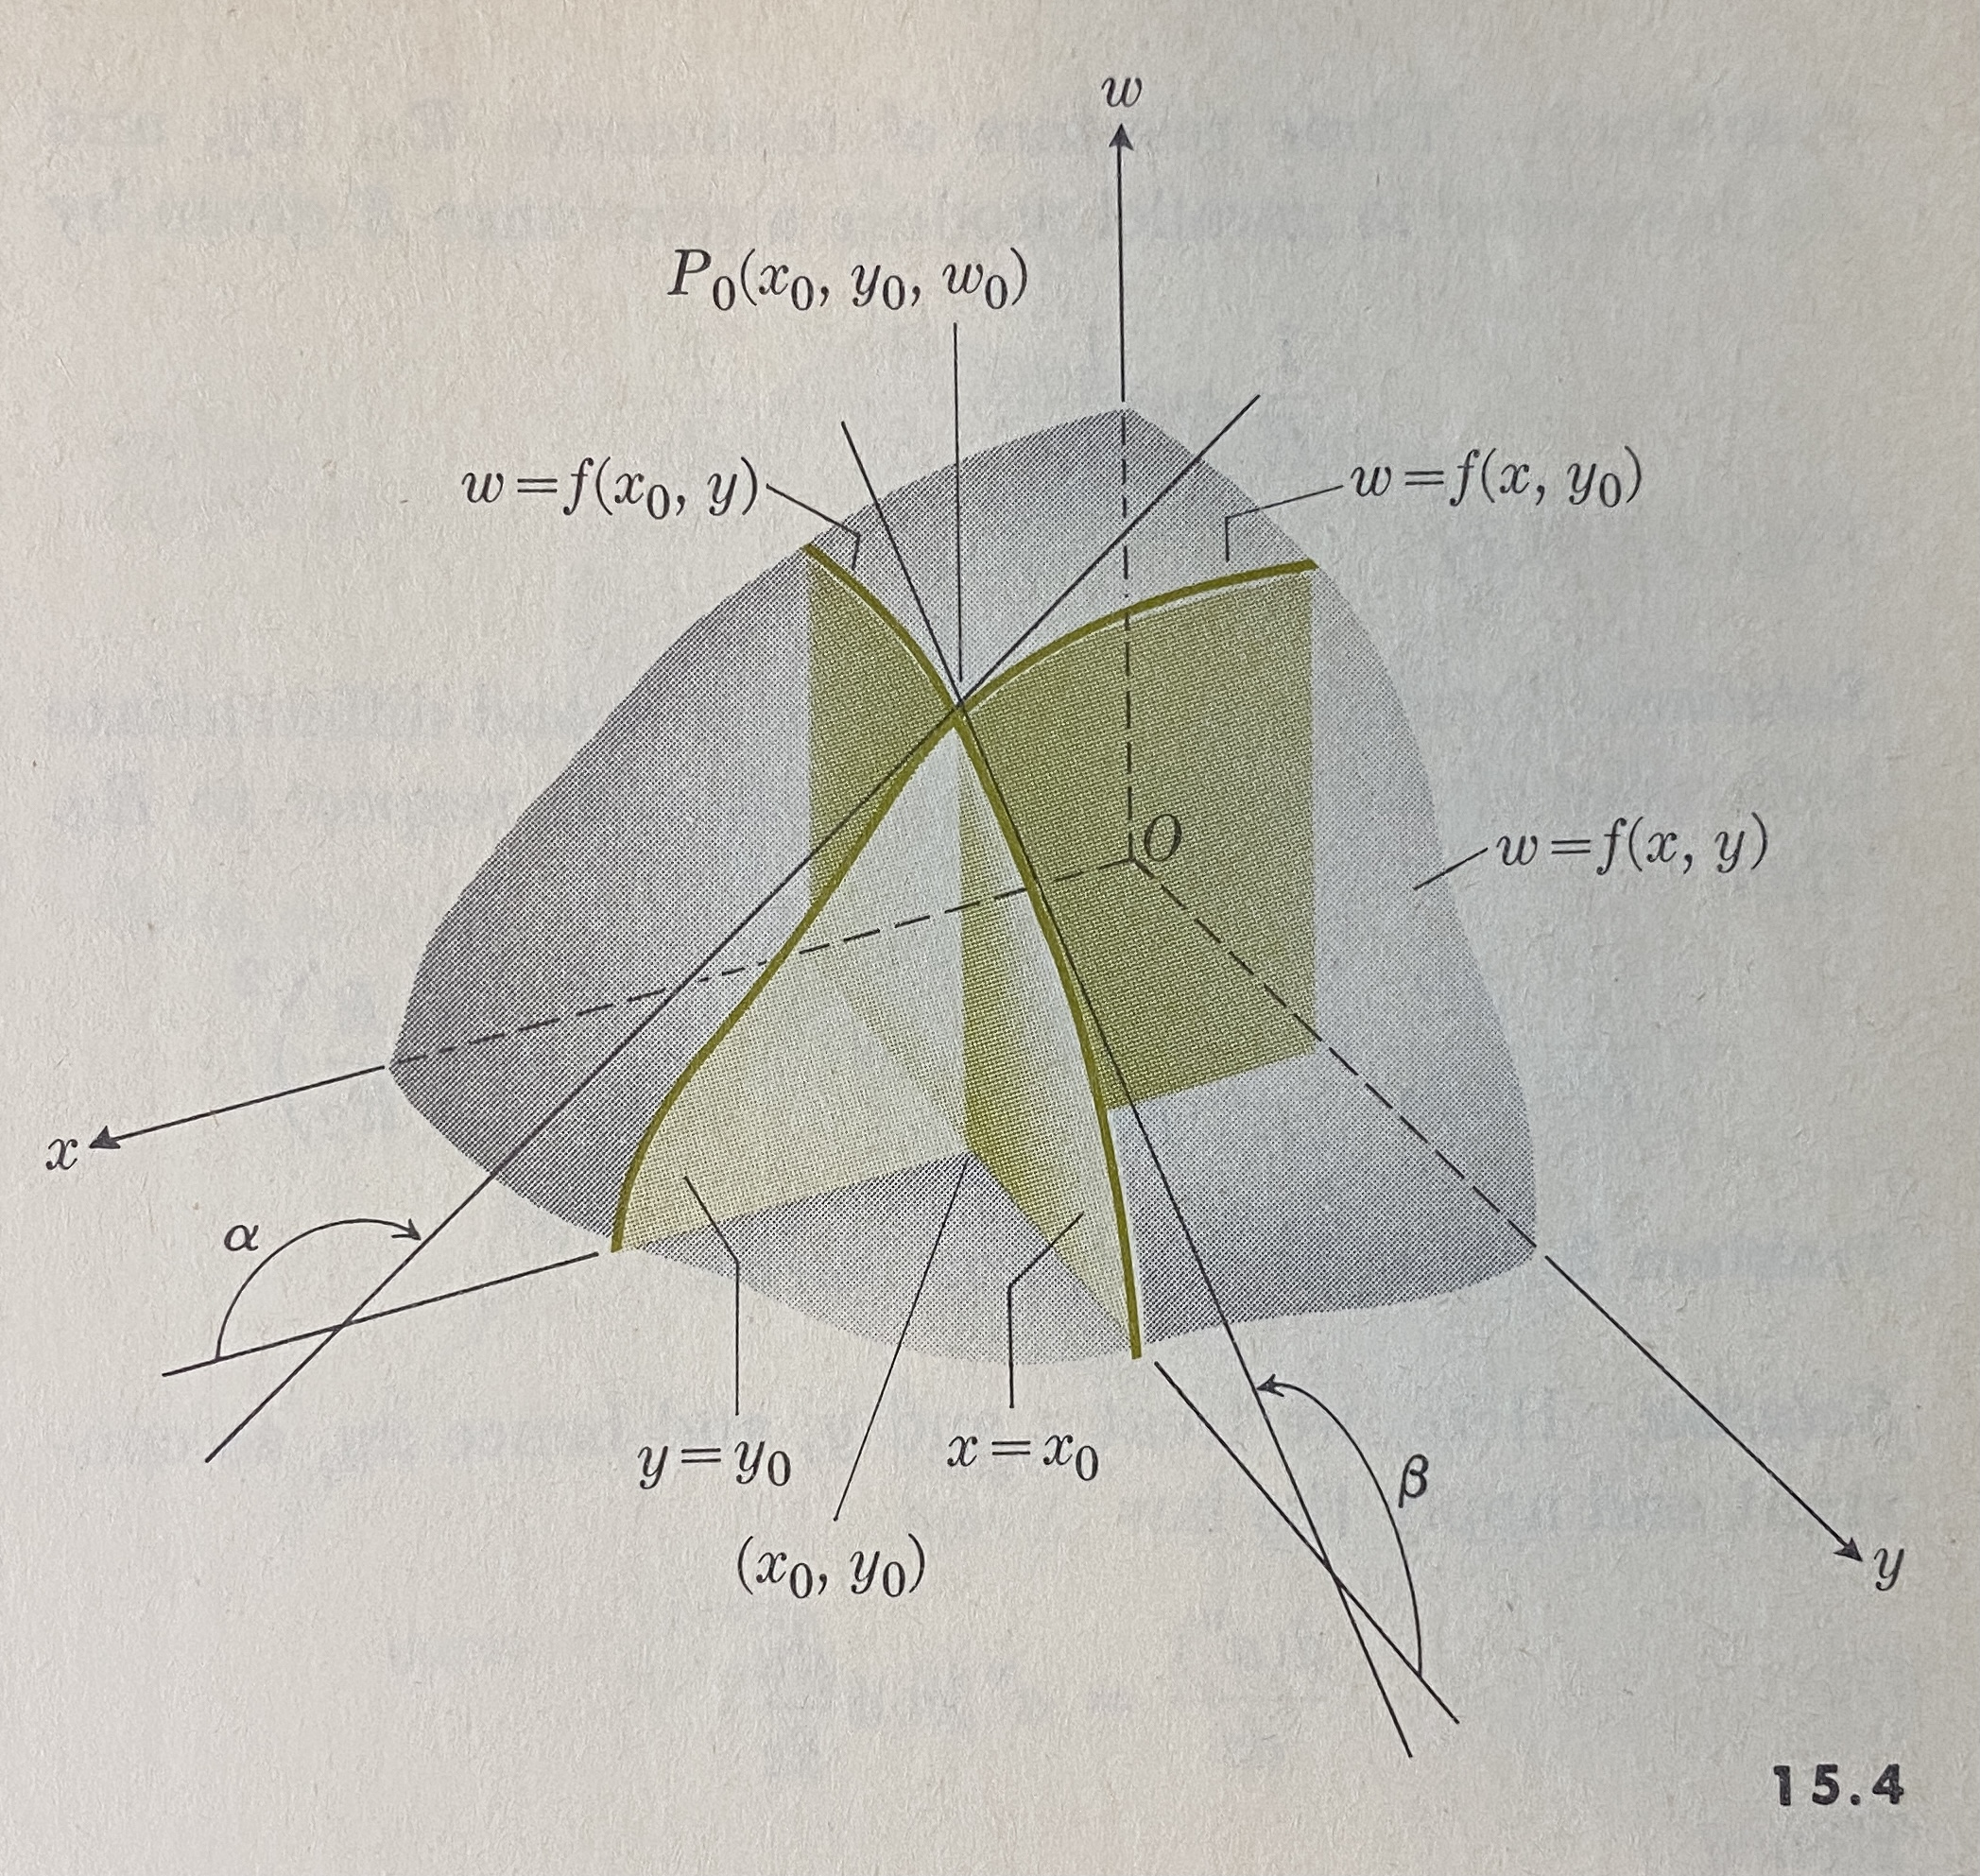
\includegraphics[width=0.4\linewidth]{ExtFiles/geometricPartialDv.jpg}
        \caption{Geometric interpretation of the partial derivative.}
        \label{fig:geometricPartialDv}
    \end{figure}
    \item As in Figure \ref{fig:geometricPartialDv}, the geometric interpretation of the partial derivative (wrt. $x$) at a point $P(x_0,y_0,w_0)$ is as the slope of the curve $f(x,y_0)$, and symetrically wrt. $y$.
    \item We can define the partial derivative with respect to $y$ similarly to how it is defined for $x$.
    \begin{equation*}
        \pdv{w}{y} = f_y(x,y) = \lim_{\Delta y\to 0}\frac{f(x,y+\Delta y)-f(x,y)}{\Delta y}
    \end{equation*}
    \item With higher order derivatives $\pdv*{w}{z}$, $\pdv*{w}{u}$, $\pdv*{w}{v}$, and more as in $w=f(x,y,z,u,v)$, we evaluate by holding all but the variable of interest constant.
    \item To denote the partial derivative at a point, we have two notations:
    \begin{align*}
        \left( \pdv{w}{x} \right)_{(x_0,y_0)}&&
            f_x(x_0,y_0)
    \end{align*}
\end{itemize}



\section{Tangent Plane and Normal Line}
\begin{itemize}
    \item \textbf{Tangent plane} (to $w=f(x,y)$ at $P_0(x_0,y_0,w_0)$): A plane $T$ such that for any point $P$ on the surface described by $f(x,y)$, as $P\to P_0$, the angle between $T$ and $\overline{PP_0}$ approaches 0.
    \item \textbf{Normal line} (to $w=f(x,y)$ at $P_0(x_0,y_0,w_0)$): The line through $P_0$ which is normal to the tangent plane to $f(x,y)$ at $P_0$.
    \item The tangent plane is determined by the lines $L_1$ and $L_2$ tangent to the curves $C_1:w=f(x_0,y)$ and $C_2:w=f(x,y_0)$; the slopes of these lines are given by $\pdv*{w}{y}$ and $\pdv*{w}{x}$, respectively.
    \item Formulae for the tangent plane and normal line follow easily after finding a normal vector $\textbf{N}$ to the plane of $L_1$ and $L_2$. To find $\textbf{N}$, we can use the cross product of the vectors $\textbf{v}_1$ and $\textbf{v}_2$ lying along $L_1$ and $L_2$, respectively.
    \begin{figure}[h!]
        \centering
        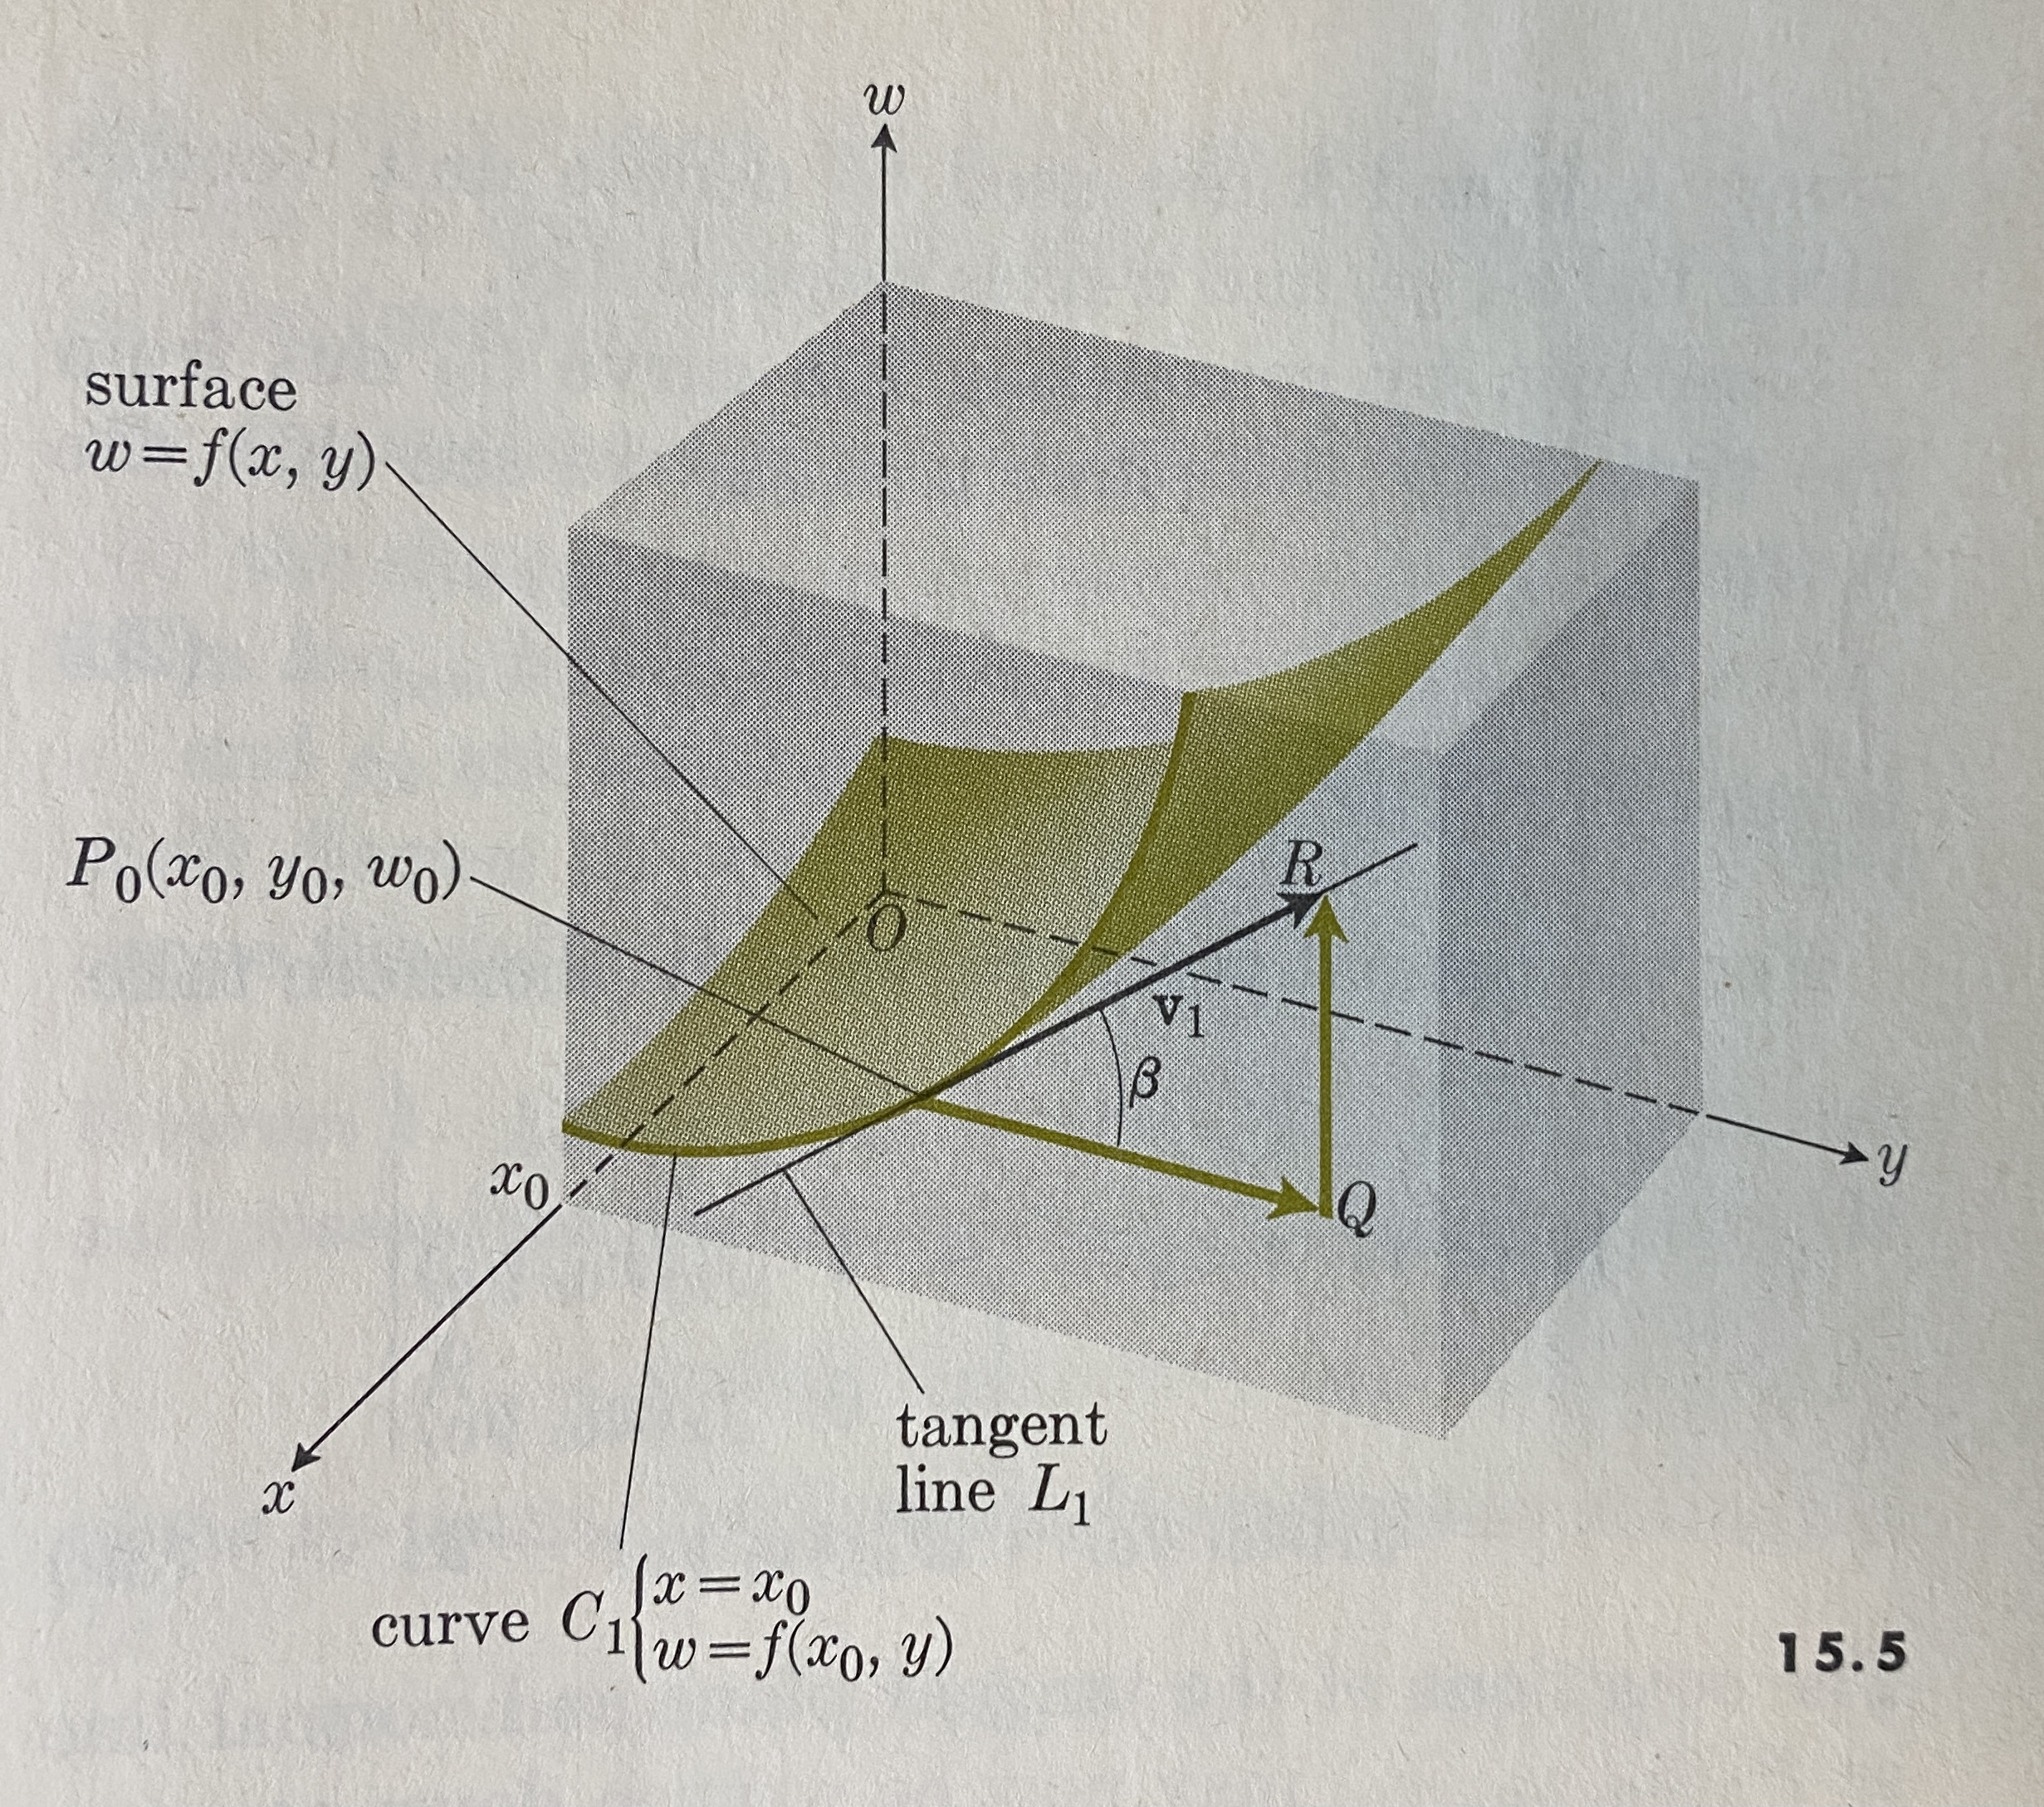
\includegraphics[width=0.4\linewidth]{ExtFiles/deriveTangentPlane.jpg}
        \caption{Deriving formulae for the tangent plane and normal line.}
        \label{fig:deriveTangentPlane}
    \end{figure}
    \begin{itemize}
        \item From Figure \ref{fig:deriveTangentPlane}, we can see that
        \begin{align*}
            \textbf{v}_1 &= \textbf{j}+f_y(x_0,y_0)\textbf{k}&
                \textbf{v}_2 &= \textbf{i}+f_x(x_0,y_0)\textbf{k}
        \end{align*}
        \item Thus,
        \begin{equation*}
            \textbf{N} = \textbf{i}f_x(x_0,y_0)+\textbf{j}f_y(x_0,y_0)-\textbf{k}
        \end{equation*}
        \item Therefore, the formulae for the tangent plane and normal line, respectively, are
        \begin{align*}
            A(x-x_0)+B(y-y_0)+C(w-w_0) &= 0&
                (x,y,w) &= (x_0,y_0,w_0)+t(A,B,C)
        \end{align*}
        where $A=f_x(x_0,y_0)$, $B=f_y(x_0,y_0)$, $C=-1$, and $t\in(-\infty,\infty)$.
        \item In vector form, if $\textbf{R}=\textbf{i}x+\textbf{j}y+\textbf{k}z$ and $\textbf{R}_0=\textbf{i}x_0+\textbf{j}y_0+\textbf{k}z_0$, then
        \begin{align*}
            \textbf{N} &= \textbf{i}f_x(x_0,y_0)+\textbf{j}f_y(x_0,y_0)-\textbf{k}&
                \textbf{N}\cdot(\textbf{R}-\textbf{R}_0) &= 0&
                    \textbf{R} &= \textbf{R}_0+t\textbf{N}
        \end{align*}
    \end{itemize}
\end{itemize}



\section{Approximate Value of \texorpdfstring{$\Delta w$}{TEXT}}
\begin{itemize}
    \item \textbf{Linearization} (of $f$ at $P_0$): The function (based off of the tangent plane)
    \begin{equation*}
        w = f(x_0,y_0)+f_x(x_0,y_0)\cdot(x-x_0)+f_y(x_0,y_0)\cdot(y-y_0)
    \end{equation*}
    \item Note that
    \begin{equation*}
        \Delta w_\text{tan} = f_x(x_0,y_0)\Delta x+f_y(x_0,y_0)\Delta y
    \end{equation*}
    meaning that to calculate $\Delta w_\text{tan}$, we need only add the tangential components; no other interaction term is needed.
    \item Important results:
    \begin{thm}
        Let the function $w=f(x,y)$ be continuous and possess partial derivatives $f_x,f_y$ throughout a region $R:|x-x_0|<h,\ |y-y_0|<k$ of the $xy$-plane. Let $f_x$ and $f_y$ be continuous at $(x_0,y_0)$. Let $\Delta w = f(x_0+\Delta x,y_0+\Delta y)-f(x_0,y_0)$. Then
        \begin{equation*}
            \Delta w = f_x(x_0,y_0)\Delta x+f_y(x_0,y_0)\Delta y+\epsilon_1\Delta x+\epsilon_2\Delta y
        \end{equation*}
        where $\epsilon_1,\epsilon_2\to 0$ when $\Delta x,\Delta y\to 0$.
    \end{thm}
    \begin{cly}
        Let $w=f(x,y)$ be continuous in a region $R:|x-x_0|<h,\ |y-y_0|<k$. Let $f_x$ and $f_y$ exist in $R$ and be continuous at $(x_0,y_0)$. Then the surface $w=f(x,y)$ has a tangent plane at $P_0(x_0,y_0,w_0)$, where $w_0=f(x_0,y_0)$.
    \end{cly}
    \begin{itemize}
        \item These results extend into finitely higher dimensions.
    \end{itemize}
\end{itemize}




\end{document}